\documentclass[border=16pt]{standalone}

\usepackage{amsmath}
\usepackage{amssymb}
\usepackage{xcolor}
\usepackage{tikz}
\usetikzlibrary{arrows.meta,positioning,fit,backgrounds,calc,decorations.pathreplacing,decorations.markings}

\definecolor{ink}{RGB}{30,40,56}
\definecolor{muted}{RGB}{104,110,124}
\definecolor{fabric}{RGB}{46,84,126}
\definecolor{fabricfill}{RGB}{223,234,244}
\definecolor{ringred}{RGB}{178,60,48}
\definecolor{hostA}{RGB}{58,110,165}
\definecolor{hostB}{RGB}{197,132,42}
\definecolor{hostC}{RGB}{82,138,80}
\definecolor{hostD}{RGB}{136,88,158}

\begin{document}
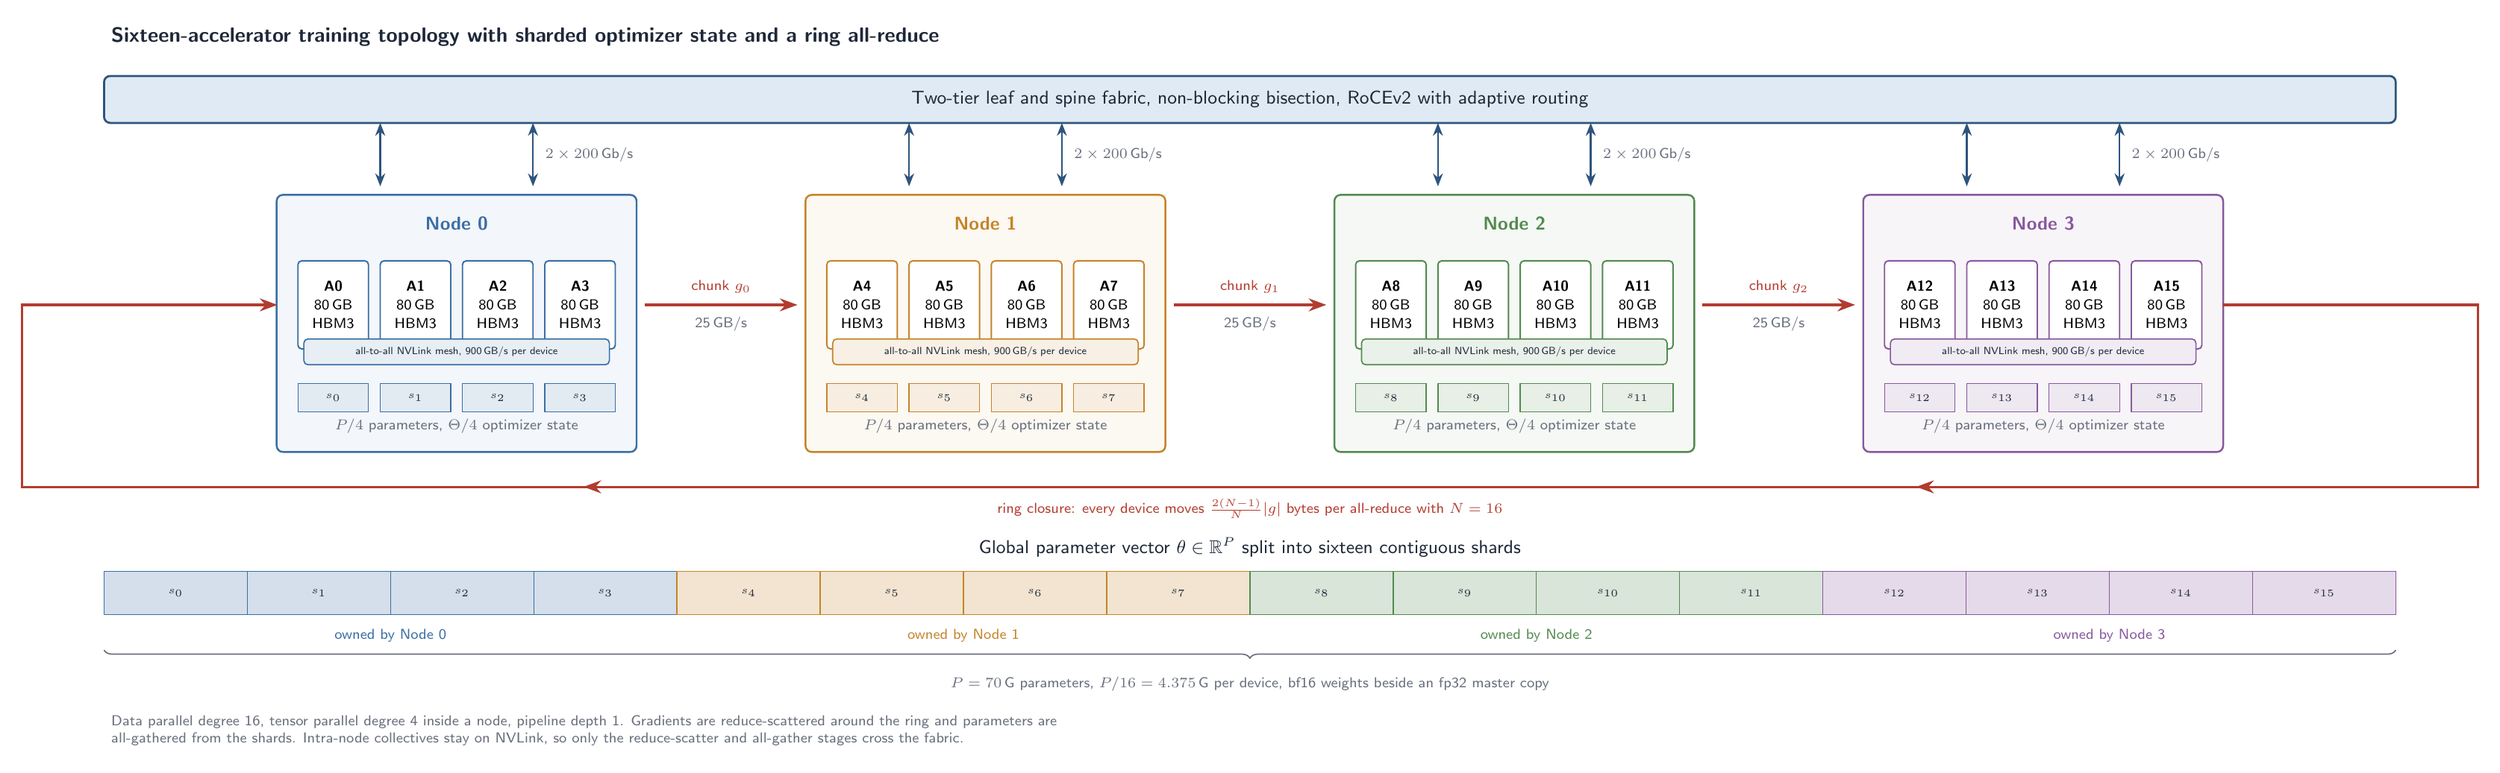
\begin{tikzpicture}[
    font=\sffamily,
    dev/.style={draw=#1,line width=0.7pt,rounded corners=1.8pt,fill=white,
      minimum width=12mm,minimum height=15mm,align=center,
      font=\sffamily\scriptsize,inner sep=1pt},
    shardcell/.style={draw=#1,line width=0.5pt,fill=#1!14,
      minimum width=12mm,minimum height=4.8mm,inner sep=0pt,
      font=\sffamily\tiny,text=ink},
    hostbox/.style={draw=#1,line width=0.9pt,rounded corners=3pt,
      fill=#1!6,inner sep=0pt},
    link/.style={{Stealth[length=2.2mm,width=1.7mm]}-{Stealth[length=2.2mm,width=1.7mm]},
      line width=0.8pt,draw=fabric},
    ring/.style={-{Stealth[length=3mm,width=2.2mm]},line width=1.1pt,
      draw=ringred},
    ringpath/.style={-{Stealth[length=3mm,width=2.2mm]},line width=1.1pt,
      draw=ringred,
      postaction={decorate,decoration={markings,
        mark=at position 0.30 with {\arrow[line width=1.1pt]{Stealth[length=3mm,width=2.2mm]}},
        mark=at position 0.70 with {\arrow[line width=1.1pt]{Stealth[length=3mm,width=2.2mm]}}}}},
    note/.style={font=\sffamily\scriptsize,text=muted,inner sep=1.5pt},
    bignote/.style={font=\sffamily\small,text=ink,inner sep=2pt},
  ]

  \def\devy{8.60}
  \def\nvy{7.80}
  \def\shy{7.02}
  \def\barl{-6.0}
  \def\barr{33.0}
  \def\barw{2.4375}

  \foreach \i/\x/\col/\name in {0/0/hostA/{Node 0},
                                1/9/hostB/{Node 1},
                                2/18/hostC/{Node 2},
                                3/27/hostD/{Node 3}} {
    \foreach \d/\dx in {0/-2.10, 1/-0.70, 2/0.70, 3/2.10} {
      \pgfmathtruncatemacro{\gid}{4*\i+\d}
      \node[dev=\col] (dev\i\d) at ({\x+\dx},\devy)
        {\textbf{A\gid}\\[1pt]\scriptsize 80\,GB\\[1pt]\scriptsize HBM3};
      \node[shardcell=\col] (sh\i\d) at ({\x+\dx},\shy) {$s_{\gid}$};
    }
    \node[draw=\col,line width=0.6pt,rounded corners=2pt,fill=\col!12,
          minimum width=52mm,minimum height=4.4mm,inner sep=0pt,
          font=\sffamily\tiny,text=ink] (nv\i) at (\x,\nvy)
      {all-to-all NVLink mesh, 900\,GB/s per device};
    \node[font=\sffamily\small\bfseries,text=\col] (title\i) at (\x,9.98) {\name};
    \node[note,anchor=north] (cap\i) at (\x,6.72)
      {$P/4$ parameters, $\Theta/4$ optimizer state};
  }

  \begin{scope}[on background layer]
    \foreach \i/\col in {0/hostA, 1/hostB, 2/hostC, 3/hostD} {
      \node[hostbox=\col,
            fit=(title\i)(dev\i0)(dev\i3)(nv\i)(sh\i0)(sh\i3)(cap\i),
            inner xsep=3.5mm,inner ysep=2.6mm] (host\i) {};
    }
  \end{scope}

  \node[draw=fabric,line width=1pt,rounded corners=3pt,fill=fabricfill,
        minimum width=390mm,minimum height=8mm,inner sep=0pt,
        font=\sffamily\small,text=ink] (spine) at (13.5,12.10)
    {Two-tier leaf and spine fabric, non-blocking bisection, RoCEv2 with adaptive routing};

  \foreach \x in {0,9,18,27} {
    \draw[link] ({\x-1.3},10.62) -- ({\x-1.3},11.70);
    \draw[link] ({\x+1.3},10.62) -- ({\x+1.3},11.70);
    \node[note,anchor=west] at ({\x+1.45},11.16) {$2\times 200$\,Gb/s};
  }

  \foreach \i/\x in {0/4.5, 1/13.5, 2/22.5} {
    \draw[ring] ({\x-1.3},\devy) -- ({\x+1.3},\devy);
    \node[note,anchor=south,text=ringred] at (\x,{\devy+0.14})
      {chunk $g_{\i}$};
    \node[note,anchor=north] at (\x,{\devy-0.14}) {25\,GB/s};
  }

  \draw[ringpath] (30.05,\devy) -- (34.4,\devy) -- (34.4,5.50)
    -- (-7.4,5.50) -- (-7.4,\devy) -- (-3.05,\devy);
  \node[note,anchor=north,text=ringred] at (13.5,5.36)
    {ring closure: every device moves $\tfrac{2(N-1)}{N}\lvert g\rvert$ bytes per all-reduce with $N = 16$};

  \node[bignote,anchor=south] at (13.5,4.22)
    {Global parameter vector $\theta \in \mathbb{R}^{P}$ split into sixteen contiguous shards};

  \foreach \i/\col in {0/hostA, 1/hostB, 2/hostC, 3/hostD} {
    \foreach \d in {0,1,2,3} {
      \pgfmathtruncatemacro{\gid}{4*\i+\d}
      \pgfmathsetmacro{\bx}{\barl + \barw*\gid}
      \pgfmathsetmacro{\bxe}{\barl + \barw*(\gid+1)}
      \draw[draw=\col,line width=0.5pt,fill=\col!22]
        (\bx,3.32) rectangle (\bxe,4.06);
      \node[font=\sffamily\tiny,text=ink] at ({(\bx+\bxe)/2},3.69) {$s_{\gid}$};
    }
    \pgfmathsetmacro{\gl}{\barl + \barw*4*\i}
    \pgfmathsetmacro{\gr}{\barl + \barw*(4*\i+4)}
    \node[font=\sffamily\scriptsize,text=\col,anchor=north]
      at ({(\gl+\gr)/2},3.20) {owned by Node \i};
  }

  \draw[decorate,decoration={brace,amplitude=4pt,mirror},draw=muted,
        line width=0.6pt] (\barl,2.72) -- (\barr,2.72);
  \node[note,anchor=north] at (13.5,2.32)
    {$P = 70$\,G parameters, $P/16 = 4.375$\,G per device, bf16 weights beside an fp32 master copy};

  \node[anchor=north west,align=left,font=\sffamily\scriptsize,text=muted]
    at (\barl,1.72)
    {Data parallel degree 16, tensor parallel degree 4 inside a node, pipeline depth 1.
     Gradients are reduce-scattered around the ring and parameters are\\
     all-gathered from the shards. Intra-node collectives stay on NVLink, so only the
     reduce-scatter and all-gather stages cross the fabric.};

  \node[anchor=north west,font=\sffamily\bfseries,text=ink]
    at (\barl,13.45)
    {Sixteen-accelerator training topology with sharded optimizer state and a ring all-reduce};

\end{tikzpicture}
\end{document}
